%%
%% This is file `sample-authordraft.tex',
%% generated with the docstrip utility.
%%
%% The original source files were:
%%
%% samples.dtx  (with options: `authordraft')
%% 
%% IMPORTANT NOTICE:
%% 
%% For the copyright see the source file.
%% 
%% Any modified versions of this file must be renamed
%% with new filenames distinct from sample-authordraft.tex.
%% 
%% For distribution of the original source see the terms
%% for copying and modification in the file samples.dtx.
%% 
%% This generated file may be distributed as long as the
%% original source files, as listed above, are part of the
%% same distribution. (The sources need not necessarily be
%% in the same archive or directory.)
%%
%% The first command in your LaTeX source must be the \documentclass command.
\documentclass[noacm,sigconf,authorversion]{acmart}
%% NOTE that a single column version may be required for 
%% submission and peer review. This can be done by changing
%% the \doucmentclass[...]{acmart} in this template to 
%% \documentclass[manuscript,screen,review]{acmart}
%% 
%% To ensure 100% compatibility, please check the white list of
%% approved LaTeX packages to be used with the Master Article Template at
%% https://www.acm.org/publications/taps/whitelist-of-latex-packages 
%% before creating your document. The white list page provides 
%% information on how to submit additional LaTeX packages for 
%% review and adoption.
%% Fonts used in the template cannot be substituted; margin 
%% adjustments are not allowed.
%%
%% \BibTeX command to typeset BibTeX logo in the docs
\AtBeginDocument{%
  \providecommand\BibTeX{{%
    \normalfont B\kern-0.5em{\scshape i\kern-0.25em b}\kern-0.8em\TeX}}}

%% Rights management information.  This information is sent to you
%% when you complete the rights form.  These commands have SAMPLE
%% values in them; it is your responsibility as an author to replace
%% the commands and values with those provided to you when you
%% complete the rights form.

\usepackage[utf8]{inputenc}
\usepackage[english]{babel}
\usepackage[margin=2cm]{geometry}
\usepackage{booktabs}\newcommand{\ra}[1]{\renewcommand{\arraystretch}{#1}}

%bibliography packages
\usepackage{natbib}
\usepackage{booktabs}
\usepackage{amssymb}
\usepackage{tabularx}
\usepackage{paralist}


\usepackage{multicol, caption}
\usepackage{wrapfig}


\usepackage{natbib}
\usepackage{graphicx}
\usepackage{array, makecell} 
\usepackage{amsmath}
\usepackage{amssymb}% http://ctan.org/pkg/amssymb
\usepackage{pifont}% http://ctan.org/pkg/pifont
\newcommand{\cmark}{\ding{51}}%
\newcommand{\xmark}{\ding{55}}%

\usepackage{caption}
\usepackage{etoolbox}

\setlength{\belowcaptionskip}{0pt}

\patchcmd{\maketitle}{\@copyrightspace}{}{}{}
\acmPrice{}
\acmISBN{}
\acmDOI{}
\acmPubDate{}
%%
%% Submission ID.
%% Use this when submitting an article to a sponsored event. You'll
%% receive a unique submission ID from the organizers
%% of the event, and this ID should be used as the parameter to this command.
%%\acmSubmissionID{123-A56-BU3}

%%
%% The majority of ACM publications use numbered citations and
%% references.  The command \citestyle{authoryear} switches to the
%% "author year" style.
%%
%% If you are preparing content for an event
%% sponsored by ACM SIGGRAPH, you must use the "author year" style of
%% citations and references.
%% Uncommenting
%% the next command will enable that style.
%%\citestyle{acmauthoryear}

%%
%% end of the preamble, start of the body of the document source.
\begin{document}
\acmConference[Project Report]{ACM Conference}{June 2021}{Lausanne,
 VD, CH}%
 
 
\title{GME to the Moon, or how r/WallStreetBets squeezed GameStop} 

\author{Atri Bhattacharyya}
\affiliation{EPFL}
\email{atri.bhattacharyya@epfl.ch}

\author{Aurel R. Mader}
\affiliation{EPFL}
\email{aurel.mader@epfl.ch}

\author{Ludovica Schaerf}
\affiliation{EPFL}
\email{ludovica.schaerf@epfl.ch}

%%
%% The abstract is a short summary of the work to be presented in the
%% article.
\begin{abstract}
  In January 2021, the Reddit community r/WallStreetBets was attributed 
  for causing a once-in-a-decade short squeeze on the GameStop stock.
  In this paper, we analyze the interactions (posts, comments) within 
  the community to determine whether the community could indeed have been
  responsible, and whether the actions of the community represent a 
  mass movement of individual players.
  % maybe a bit to shallow
\end{abstract}

%%
%% Keywords. The author(s) should pick words that accurately describe
%% the work being presented. Separate the keywords with commas.
\keywords{GME, Reddit, Network Analysis, Stock Market, Regression Analysis}


%%
%% This command processes the author and affiliation and title
%% information and builds the first part of the formatted document.
\maketitle

\section{Introduction}

Communities on social media have the power to affect large-scale social movements since social
media allows people to connect far beyond their local communities, and with unprecedented speed. % source?

In this paper, we investigate the role of a community on the social media platform Reddit, r/WallStreetBets (r/WSB), in the short 
squeeze of the publicly traded stocks of GameStop, a retailer of video games with physical stores across the world.

In January 2021, the stock prices of GameStop (\$GME stock) saw a bizarre price movement.
Whereas the stock had consistently traded for less than \$10 over the previous year, the 
price rose meteorically, peaking at \$347 \cite{umar2021tale}.
Being a physical retailer in the age of giant digital game distributors such as Steam and 
Epic Games, GameStop was widely regarded as a relic of the past and predicted to slowly 
fade into irrelevance (parallels exist to the decline of the video rental chain Blockbuster, being supplanted by video streaming services such as Netflix).

There were two major factions betting on \$GME. 
On one side, hedge funds had made short contracts amounting to more than 140\% of \$GME's stocks~\cite{shortlosses2021}.
On the other side, prominent members of the r/WallStreetBets community encouraged retail investors
to buy the stock en masse, believing it to be undervalued~\cite{chohan2021counter}. 
During the ensuing price spike, it is reported that short sellers lost over \$6 billion~\cite{shortlosses2021}. 
While long term stock holders from the Reddit community made significant gains, a large number 
of Reddit users who entered the market near the peak have suffered large losses.

Our interest in the \$GME short squeeze revolves around understanding the dynamics of the 
Reddit community (called a \emph{subreddit} in Reddit terminology). 
To counter the billions invested by hedge funds, the investments from the subreddit would 
have to match it. 
Given the limited means of retail investors, a large number of them would have to pool resources
to cause the short squeeze, as often claimed~\cite{chohan2021counter, umar2021tale}. Or the short squeeze might also have been driven and orchestrated by a few financially strong actors.
This introduces our first research question: whether the /r/WallStreetBets community is dominated 
by a few highly influential individuals, or whether the community is more egalitarian and 
influenced by a larger number of members.

For our second research question, we ask whether the actors in the subreddit were actually 
responsible for the short squeeze, and whether the publicly available information from the 
subreddit can be used to measure the impact of the subreddit on price fluctuations of \$GME.
%We want to look into whether people interacting or generating discussion in the 
%subreddit correlates with price changes in the stock.


\section{Literature Review}
The short squeeze of the Gamestop stock has been vastly covered by the media and recent academic research~\cite{chohan2021counter, intradaygamestop, long2021just, burnette2021were, lyocsa2021yolo, umar2021tale}. Prior research analyzes the short squeeze by looking at the interest in the GME stocks as visible on Google trends~\cite{intradaygamestop, lyocsa2021yolo} and pays special attention to the influence of Google trends on the trading volume of the GME stock~\cite{intradaygamestop}. The influence of the subreddit r/WallStreetBets in the GME phenomenon has  been  investigated before by trying to quantify the role of the subbredit in the short squeeze~\cite{lyocsa2021yolo}. Furthermore, other research already uses twitter data, as e.g. twitter posts with corresponding hashtags,  to measure the interest of the online community concerning the GME stock~\cite{umar2021tale}. \par
 In line with this research, this paper computes a number of features to determine the influence of the subreddit on the stock price of GME. Other research focuses on the general role of social media in coordinating such a mass event, and explains its counter-hegemonic motivation~\cite{chohan2021counter, burnette2021were}. Long et. al.~\citep{long2021just} studies the sentiment of the comments published on r/WallStreetBets to trace its role in the development of the short squeeze. To the best of our knowledge, no research in the direction of an organic computational analysis of r/WallStreetBets in the context of metoric rise in the GME stock price has been conducted before.\par 

In the broader context of Reddit, previous research has drawn upon methods of Social Network Analysis (SNA), sentiment analysis, topic detection and regression analysis to determine the behavior of a specific subreddit or the interconnections among reddit communities~\cite{cai_characterizing, moessner2018analyzing}. Similarly, this analysis makes use of SNA and regression analysis to capture a number of characteristics of the subreddit. \par

Lastly, Boylston et. al.~\citep{boylston2021wallstreetbets} analyzes the dynamics of the r/WSB subreddit. Among the dynamics considered, it reconstructs the source of trust that is established among members, evidencing the different roles inside the community and characterizing the specific jargon used. 

\section{Data}

\subsection{Data Collection}

\begin{table}
    \centering
\begin{tabularx}{\linewidth}{l | l }
    \hline
    Field            & Description \\ \hline \hline 
    Author           & User ID of post/comment author \\ \hline
    Created UTC      & Timestamp of creation data and time \\ \hline
    ID               & Unique object identifier \\ \hline
    Score            & Post rating based on up/downvotes \\ \hline
    Subreddit ID     & Subreddit a post/comment was made in \\ \hline
    All awardings    & Lists awards given to the post/comment \\ \hline
    URL              & URL of linked content \\ \hline
    Over 18          & User/moderator tagged sensitive content \\ \hline
    Link Flair Type  & User-marked flair or topic for the post \\ \hline
    Parent ID        & ID of parent post/comment for comments \\ \hline
    Seft Text        & Text body of text post \\  \hline
    Body             & Text content of comment \\ \hline
\end{tabularx}
    \caption{Metadata fields available in reddit dataset}
    \label{tab:reddit_meta}
\end{table}

To analyze the interactions within a Reddit community (subreddit) for determining their effect on stock prices, we collected publicly available data from Reddit using a third-party API (PushShift). 
The data corresponds to publicly visible posts and comments made by users on the subreddit.
The collected data covers the period of highest volatility of the GameStop stock price, extending from January $1^{st}$ 2021 to March $17^{th}$ 2021. Financial data describing the hourly stock price of GME was collected for the same time period using the Yahoo finance API \cite{berube2007retrieving}.

\paragraph{Introduction to Reddit data}
Of the different interactions between users available on Reddit, posts, comments, upvotes and awards are publicly available. 
Other interactions, such as direct messages, are private and therefore not available via the Reddit API. 
Interactions happen within communities (aka subreddits) dedicated for a particular topic (for e.g., music, gaming and videos). 

Users initiate activity within a community by authoring posts. 
Posts come in two varieties: link posts and text posts. 
Link posts contain a title and a link to some content, often images, videos, news stories or other posts. 
Text posts contain a title and text written by the author. The contents of the text are generally unrestricted, and can contain links too. 
Posts which link to images and videos often contain content which is humorous in nature, such as memes. 
A significant portion of posts in many subreddits comprise memes.

Text posts, or those linking to news articles are often more serious, and used for either sharing news which concerns the community, or sharing personal opinions, explanations and analyses.

For each post on a subreddit, user interactions continue in the form of comments which form a tree structure. 
Top-level comments directly address the post, whereas children are comments on previous comments. 
Comments are free-form text fields and can contain discussions, links or both. 

Users are allowed to express their like or dislike of posts and comments with the up/downvote feature. 
Each user is allowed to contribute a single up/downvote to every comment or post. 
Posts and comments, therefore, have a score which is the resulting difference of upvotes and downvotes. 
Visitors to subreddits often sort posts by "Top" (highest score within a period) or "Hot" (score/time), both of which result in posts with high scores gaining higher visibility. 

Finally, communities contain moderators who work to enforce community policies. 
As part of their arsenal, they are able to delete posts and comments which violate rules.
Users are also allowed to delete their own posts and comments.

\paragraph{Basic data description}
We collected data using the API available from pushshift.io, which mirrors reddit data. 
Compared to the API natively offered by Reddit, this enabled us to search for posts within a start and end-point in time. 
Both Reddit and Pushshift enforce a limit of 1000 items in the response for any query. 
Having the ability to dynamically query posts within a time-frame allowed us to download the entire post history ($900'100$ posts) over multiple queries. 

The scoring system of Reddit also ensures that a vast majority of posts receive little to no attention. 
From the list of all posts, we choose to ignore posts which have less than a single comment and a single upvote. 
We believe that such posts have no impact on the community, and can be safely ignored without affecting our analyses. 
Of the $138'364$ posts which remain, we also discard posts which have been deleted. 
Unfortunately, it is entirely possible that a deleted post enjoyed a period of popularity before its deletion, and that it affected the community sentiment. 
However, the post's data are not available from either the Reddit or Pushshift API, so our data set remains lacking in this respect. 
Finally, we have $80,283$ posts remaining, used for the analysis. 

For each post, we also fetch its list of comments. 
In total, our data set include $15,371,115$ comments.
Fetching comments include separately querying for children of every previously fetched comment, and is a time-intensive process.
Each post and comment object includes metadata, of which particular fields are shown in \autoref{tab:reddit_meta}.
A basic exploration of the data, and summary statistics are shown in \autoref{sec:summary_stats}.


\section{Methods}

\subsection{Social Network Analysis}
Social Network Analysis (SNA), as shortly covered in the Research Context, is a widely adopted technique that emerged from the social sciences and nicely lends itself to the study of online social networks~\cite{knoke2019social}. SNA is based on the study of interactions between players inside a system and is enriched by a large variety of statistics designed specifically for the technique. In this study, the network is built considering the users of the subreddit as nodes and tracing an edge for each connection between one user and another when the first user has commented on the other user's post. In this sense, the paper adopts a directed graph as basic network structure. 

The goal of this method is to answer the first research question. Investigating connections between users is here aimed at determining whether the structure of the subreddit creates the possibility of a mass phenomenon. To be a mass phenomenon, the subreddit needs to exhibit three necessary aspects:
\begin{inparaenum}[\itshape i\upshape)]
\item the structure of the r/WSB should mirror that of a tight community,
\item transmission of information between users should be quick, enabling trust, and 
\item users should cover a variety of different roles, each with diverse key players.
\end{inparaenum}

In order to detect whether a community is tight, the following hypotheses should hold. The average degree of the network\footnote{For more information on the network statistics mentioned in this section, refer to~\cite{knoke2019social}}, encoding the average number of links from/to a user, should be high. This would indicate that users are, on average, connected to many other users and can, therefore, organize efficiently a mass phenomenon. Furthermore, the overall density of connections in the network (the number of actual connections over the total possible connections) should also be rather high, showing that the amount of total connections is suited for a large mobilization of users. The number of reciprocated links should also ideally be high as it manifests the presence of bidirectional interactions during the event. Finally, similarly to real world networks, a giant component is to be expected that demonstrates that most of the users in the network have interacted with each other~\cite{knoke2019social}. The global amount of connections should also be accompanied by a high clustering coefficient (number of closed triplets over the number of triplets in the network), for which even local structures are highly connected.

For the short squeeze to have been a mass phenomenon, numerous members of the community need to have bought shares. For this to have happened, the users need to have trusted in this investment. This paper assumes that one of the reasons that pushes users to trust in the investment is if the members promoting it are, in some way, related to the users themselves. This implies that the distance from one user to another should on average (average shortest path) be low, so that a user is more likely to have come in contact with the people posting about the investment. Accordingly, the maximum distance (diameter) should also be low.

Although it is to be expected that a few users were most active in the community and in the event, to determine whether these were 'sharks' who monopolized the discourse or merely some more proactive users, this project bases its analysis on the types of key players and their roles in the network. Firstly, we assume that the discourse over this event should be created at different levels inside the community: gatekeepers should be spreading the information, visible figures should be promoting it, and common users reacting to it and 'pumping the hype'. Two metrics detecting the gatekeepers of the community were used. The first is closeness centrality, which ranks users by the average number of steps required for them to reach every other user in the network and therefore yields the users who are closest to all other users; the second is betweenness centrality, which returns users who appear most often in the shortest paths between any two users. These encode two different types of gatekeepers and should, therefore, also extract different central figures in networks that are characterized by different key players. To detect which were the visible figures in the event the HITS algorithm was used~\cite{kleinberg1999hubs}. This detects the authorities of a network (users who are often linked to, and who are, therefore, visible), and hubs (users who link to many other users, representing the most active 'common users'). Comparing among the resulting sets of popular users and determining how different these are is considered by this paper a means to determine how varied the number of proactive users in the event actually was.


\subsection{Time series Forecasting with Ordinary Least Squares (OLS)}
To assess the cross-correlation and a possible relation between the activity on the r/WSB subreddit and the meteoric rise in the stock prise of the GameStop (GME) stock,  an ordinary least squares (OLS) regression model is employed. OLS regression models are commonly used in economical and financial analysis to predict time series or more specifically to 'forecast' time series~\cite{stock2015introduction}. Although OLS models used to forecast time series do not offer any causal interpretation, they still show the relation between time shifted variables and might encode interesting information~\cite{stock2015introduction}. \par
To analyse the effect of the activity on the r/WSB subreddit onto the price change of GME, we regress some features modeling the activity in the financial forum onto a time lagged price change. The most granular financial data at our disposal is the hourly stock price of GME. The resulting time series thus consists of the hourly change of the GME stock price. To ensure that the time series is not stationary\footnote{A stationary time-series does not have a time-dependent structure, potentially leading to a spurious regression} a Augmented Dickey-Fuller test has been conducted~\cite{mushtaq2011augmented}, which indicates that our time series is indeed non-stationary (p-value: 0.000588). \par
To model the time dependence between our independent variables $X$ and our dependent variable $y$ correctly, a time lag of one hour has been implemented. Thus our resulting regression models the effect of our explanatory variables $X_t$ in time t onto our dependent variable $y_{t+1}$ in time $t+1$. Given that the stock marked is closed in the night and during the weekends, the explanatory variable $X$ does not always encompass the same period of time. Time fixed effects, e.i. weekend and night fixed effects, are use to control for this difference in the time span of observation. \par
The resulting regression then measures the effect of activity on r/WSB in period $t$ onto the price change of the GME stock in period $t+1$. To model the activity on r/WSB in period $t$ several features have been created. The most naive feature consists of the aggregated number of post discussing the GME stock in period t. To filter post which discuss GME, only post have been consider which clearly mention GME, GameStop or another GameStop synonym in their titles (in total 24'919 posts). In another regression the post have been differentiated according to their self flagged topic (see Table \ref{tab:reddit_meta}), in either discussion post (in total 8'110 pots) or reactionary posts\footnote{Consisting of all other self tagged flair beside 'Discussion'} (in total 16'809 pots). Here we assume that posts might have a different effect according to the nature of the post. In another regression specification, the posts are weighted according to the number of comments they generate. Therefore, we weighted the number of discussion and reaction posts in period $t$ by interacting them with the z-normalized number of comments they cause. A last regression specification also comprises two more covariates, which are the z-normalized post score and the average sentiment of the post title as determined by the NLTK Vader sentiment analyzer~\cite{hutto2014vader}. 
The final regression formulation is described below: 
\begin{small}

\begin{equation*}
\begin{aligned}
\Delta GME \, Price_{i,t+1} = \beta_0 + \beta_{1}Discussion_{i,t} + \beta_{2}Reaction_{i,t} +\\ \beta_{3}Comments_{zNorm, i,t}*Discussion_{i,t} + \\   
\beta_{4}Comments_{zNorm,i,t}*Reaction_{ i,t}  + \beta_{x}X_{i,t} + e_{i,t}
\end{aligned}
\end{equation*}

\end{small}

Where $ \Delta GME \, Price_{i,t+1}$ is the price change in the GME stock in one hour, $Discussion_{i,t}$ is the absolute number of discussion post in period $t$, $Reaction_{i,t}$ is the absolute number of reaction post in period $t$, both variables are interacted with the z-normalized number of comments denoted by $Comments_{zNorm, i,t}$. $X_{i,t}$ signifies the aforementioned covariates and $e_{i,t}$ the error of the model.

\section{Results}

\subsection{Summary Statistics}
\label{sec:summary_stats}

\begin{figure}[h!]       
    \includegraphics[width=0.9\linewidth]{figures/post_count.pdf}
    \caption{Number and types of posts per day.}
    \label{fig:posts_time}
\end{figure}

\begin{figure}[h!]       
    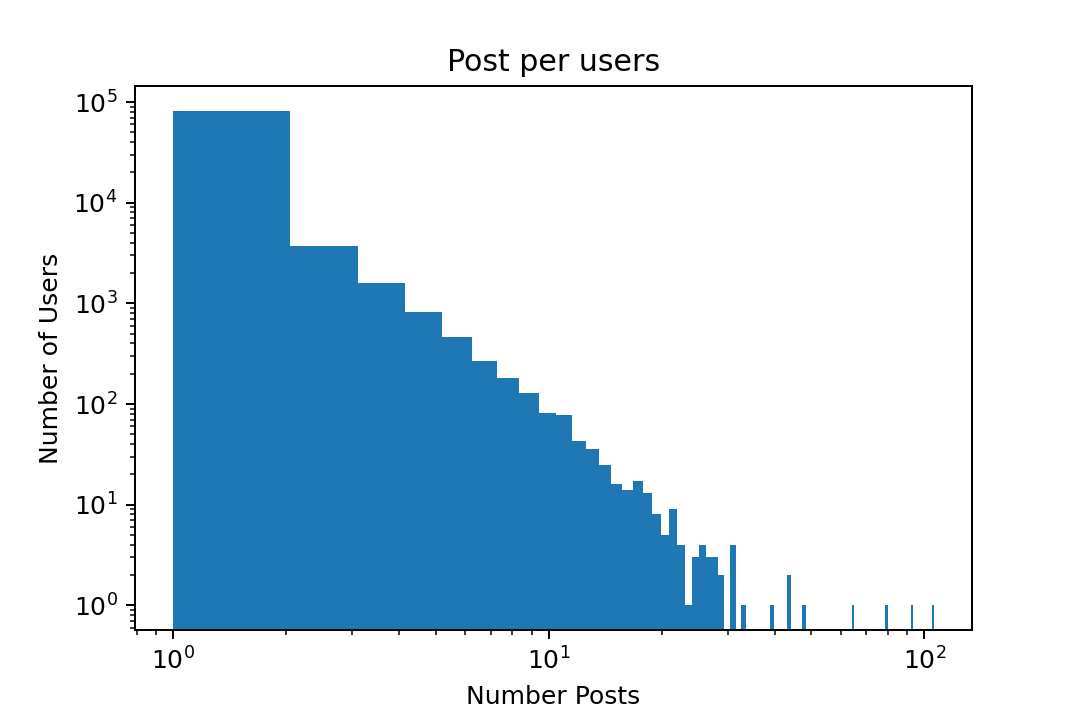
\includegraphics[width=0.9\linewidth]{figures/posts_per_user.png}
    \caption{Complementary cumulative distribution function of posts per user.}
    \label{fig:posts_per_user}
\end{figure}

This section briefly characterizes activity on the subreddit over the period of collected data.
\autoref{fig:posts_time} plots the number of posts per day over the observation period. We can see a massive rise in the 
number of posts following the short squeeze, around day 30.
This period of high activity also was the period of the highest volatility of the stock's price.
During this period, a high fraction of posts were text posts, indicating that the subreddit's userbase wanted to make their 
voices heard.
However, we can see that the vast majority of users make a low number of posts, and that only a few hundred users make more 
than 10 posts (\autoref{fig:posts_per_user}). More summary statistics and plots can be found in the Appendix.


\subsection{Network Analysis}
Following the specifics in the Methodology, a directed network with 637'395 users and 2'039'746 links (comments on posts) was built. This included on average 3.20 comments per post. Due to computational limitations, very few statistics could be run on the full network in a reasonable time-span. For this reason, a subset of the network was selected. A section of this subgraph can be seen in Figure \ref{fig:net}. This was done sampling 30'509 random users and inducing the subgraph on these nodes. The resulting network has 103'761 links and 3.40 comments per post. This method was chosen as it maintained the computed statistics (such as density, average degree, average shortest path) similar to those of the original network. 

\begin{figure}[h!]
    \centering
    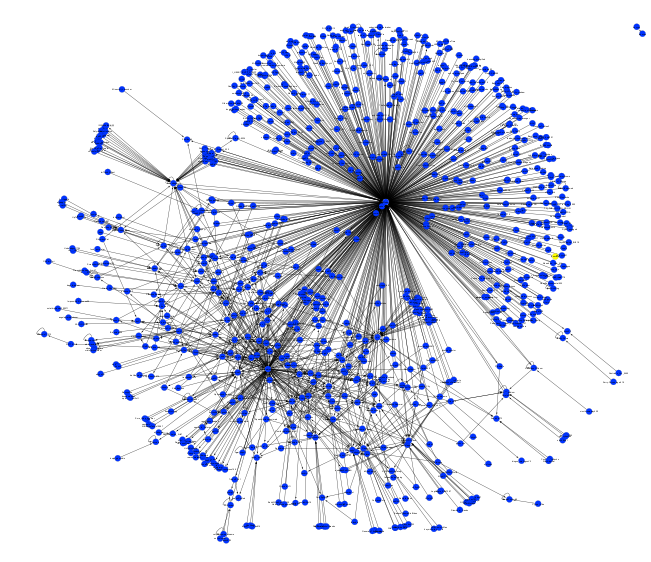
\includegraphics[width=0.7\linewidth]{figures/reddit_network_2000.png}
    \caption{Visualization of a random subset of the network.}
    \label{fig:net}
\end{figure}
On this subnetwork, the three components which characterize for us a mass phenomenon were analyzed. All the statistics of the network were computed using the python library \texttt{networkx} and reported in Table \ref{tab:stats}. Regarding the first set of hypotheses, the average degree computed is 3.40. Looking at Figure \ref{fig:deg_distr}, the degree distribution of the network follows a Zipf distribution (here note that the plot uses both logarithmic axes). This indicates that, while few users (possibly bots and moderators) have extremely high degrees, most users have about 0-10 neighbors. Being the average number of connections between 3 and 4 users and considering that this stays largely above 1 even with all the novices in the network who have none to 1 connections, this number appears rather high. However, the density of the network is barely 0.01 and the reciprocity rate 0.01. These two measures, although contradicting the hypotheses of a tight community, can be explained by the nature of the subreddit, where users do not know each other on a personal level and are, therefore, unlikely to interact with each other if not for interest in a specific post. Tracing the connected components of the network, a giant component of 23'870 nodes\footnote{This is to be expected a the average degree is greater than 1 and lower than $ln(N)$ where $N$ is the number of nodes} was detected, in accordance to the hypothesis. Moreover, the clustering coefficient is 0.23, indicating that, at a local level, about 23\% of the connections between any three users of which two are connected are complete. This is rather high considering that, in a random graph, this would be barely $\frac{3.4}{2039746}$~\cite{knoke2019social}.  

\begin{figure}[h!]       
    \mbox{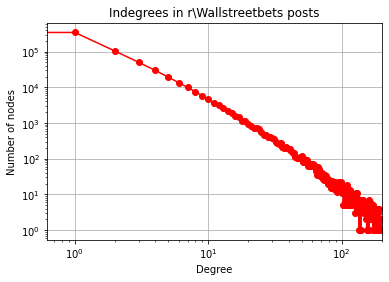
\includegraphics[scale=0.28]{figures/distribution_network.png}}
    \mbox{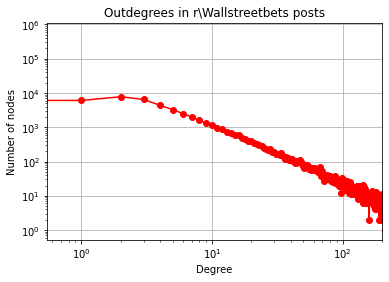
\includegraphics[scale=0.28]{figures/distribution_network_out.png}}
    \caption{Left: In-degree distribution on a loglog plot, Right: Out-degree distribution on a loglog plot.}
    \label{fig:deg_distr}
\end{figure}

The two metrics that encode the speed of the 'trust' channel in the network are both largely in accordance to the hypotheses. The maximum separation between two users in the subreddit is only 8 steps and the average is only 2.67. This is remarkably small when compared to Milgram's coefficient~\cite{travers2011experimental}, 6, and to the coefficient in Online Social Networks where it is about 4~\cite{szule2014lost}. 

\begin{table}
 \begin{center}
 \resizebox{0.4\textwidth}{!}{ 
 \begin{tabular}{|l|l|l|}
  \hline
  &\textbf{ Full-graph random subgraph}\\
  \hline
  Number of nodes & 30509 \\
  \hline
  Number of edges & 103761 \\
  \hline
  Average degree & 3.40 \\
  \hline 
  Diameter & 8 \\
  \hline
  Average clustering & 0.23 \\
  \hline
  Reciprocity & 0.01  \\
  \hline
  Average shortest path length & 2.67 \\
  \hline
  Number of communities & 6626 \\
  \hline
  Mean size of communities & 4.6 \\
  \hline
 \end{tabular}
 }
\end{center}
 \caption{Table containing statistics for the subnetwork.}
 \label{tab:stats}
\end{table}

Finally, the results on the roles and key players of the network were the most arduous to interpret. Table \ref{tab:central} shows the most central nodes according to the four centrality measures listed in the Methodology. The two measures encoding gatekeepers identify somewhat different users. Furthermore, the visible figures seem to be a summary of the most important gatekeepers. These include, among the top 20, Keith Gill (deepf******value), who was certainly one of the key actors in the network. These central users, when looking at actual posts, tend to orient the discussion towards recapitulations of the market, comment on important headlines and communication of crucial information to the community. The common users identified by the hubs are completely different from the others and, looking closely at the types of posts by these users, they reflect on their emotions, they show hype for GME and talk about their investments. The fact that the key players are different for each metric and cover different roles to propagate information, is a good indication that the community is not ruled just by few 'sharks', but rather different actors participate in different ways in the event.
Looking more in depth into the community, one can see that moderators and bots cover very prominent roles in the community (as can be seen in Table \ref{tab:central}, where the first two positions are always covered by either of the two). These two roles, interestingly, appear in all four metrics, indicating that the two roles are not most central in either specific way, rather, they are as present inside the network in different ways just as normal actors of the network. 

\begin{table}
 \begin{center}
 \resizebox{0.5\textwidth}{!}{ 
 \begin{tabular}{|l|l|l|l|l|}
  \hline
  \textbf{Degree centrality} & \textbf{Closeness centrality} & \textbf{Authorities} & \textbf{Hubs} \\
  \hline
  MotorizedD*****Canoe & MotorizedD*****Canoe & MotorizedD****Canoe & \textit{MangoManYummy} \\
  \hline 
  \textit{theycallmeryan} & \textbf{zjz} & \textit{theycallmeryan} & \textit{nosalute}\\
  \hline
  Bundaga & Tradergurue & \textbf{zjz} & giantwashcapsfan8\\
  \hline
  speakinexistencebro & Tradergurue-Prize & junaidminshad & FaithlessnessFree331\\
  \hline
  Tradergurue & MIA4real & MIA4real & disneysinger\\
  \hline
 \end{tabular}
 }
\end{center}
 \caption{Table containing top central nodes of the network. Not considering  OPINION\_IS\_UNPOPULAR and AutoModerator which are always the most central (except for Hubs). The first is a moderator while the second is an automatic moderator. When a user is a moderator in the table it is bolded, when it is a bot it is highlighted in italics.}
 \label{tab:central}
\end{table}

\begin{small}
\begin{table*}[ht]
\centering
\ra{1.3}\begin{tabular}{@{}lrrrrrrrr@{}}
\hline
& \multicolumn{7}{c}{Dependent Variable: Hourly Change in Stock Price GME (N=350)} \\
\cmidrule{2-9}
& \makecell{GME Mentions} & p-value & \makecell{Differentiation of \\ Post type} & p-value & \makecell{Differentiation of \\ Post importance} & p-value &  \makecell{Differentiation of \\ Post importance \& Covariates} & p-value \\
\hline
GME Posts &  0.0092*** & (0.003)  &  &  & & & &\\
GME Discussion Posts & & & 0.1686** & (0.027)  & 0.9120*** & (0.000) & 0.6975*** & (0.000) \\
GME Reaction Posts & & & -0.0830** & (0.016) & -0.4741*** & (0.000) &  -0.3610*** & (0.002) \\
Comments z-Normalized & & & & & -0.0890 & (0.918) & -0.0621 & (0.943) \\
\makecell{Comments z-Normalized \\ $*GME \, Discussion \, Posts$} & & & & & 2.7308*** & (0.000) & 2.0279*** & (0.003)  \\
\makecell[l]{Comments z-Normalized \\  $*GME \, Reaction \, Posts$} & &  & & & -1.4197*** & (0.000) &  -1.0802*** &  (0.005)   \\
\makecell[l]{Weekend/Night \\ Fixed Effects} & \cmark  & & \cmark  & & \cmark  & & \cmark & \\

Other Covariates & \xmark & & \xmark & & \xmark & & \cmark & \\
\bottomrule
Df Model  &  3 & & 4 & & 7 &  & 13 & \\
R-squared & 0.057 & & 0.147 & &  0.203 & & 0.230 & \\
Adj. R-squared & 0.049 & & 0.137 & & 0.186 & & 0.200 & \\
F-statistic &  7.020 & & 14.81 & & 12.41 & & 7.702 &  \\
\bottomrule
\addlinespace[1ex]
\multicolumn{3}{l}{Significance levels: \textsuperscript{***}$p<0.01$, 
  \textsuperscript{**}$p<0.05$, 
  \textsuperscript{*}$p<0.1$}
 
\end{tabular}
%\caption{}
 \caption{Results of OLS Regression: Forecasting activity on r/WSB onto GME stock price change}
 \label{tab:ols_reg_results}
\end{table*}
\end{small}

\subsection{Time Series Forecasting Results}
By implementing the described time series forecasting OLS regression model we obtain Table \ref{tab:ols_reg_results}. Table \ref{tab:ols_reg_results} describes four different estimated regressions with an increasing number of features used to explain the dependent variable. The first regression  indicates that there is a significant positive effect of the number of GME posts in period $t$ onto the price change in period $t+1$. However, this effect seems to be rather small. The second regression differentiates the type of post into discussion posts and reaction posts. Here it becomes evident that discussion posts have a significant positive effect, while reaction posts have a significant negative effect onto the price change in the next hour. Interacting the discussion and reaction posts with the z-normalized number of comments per post in the third regression increases the magnitudes of the discussion and the reaction posts coefficients. Thus we see that per discussion post with one standard deviation more than average comments the stock price increases by 2.7 dollars. The last regression uses the in the method section explained covariates to explain the change in stock price. In this regression all discussed coefficients point into the same direction and are still highly significant, they decreased however in magnitude. \par
Analyzing the obtained results, we observe some interesting trends. First, we clearly see that post on the r/WSB subreddit mentioning GME have a significant effect onto the change in stock price in the next hour. This effect seems to differentiate according to the type of the post. Discussions seem to lead to an increase in stock price while reactionary post are correlated with a decrease in stock price. Furthermore, the magnitude of those effects seems to strongly vary with how much attention the posts get, as expressed by the amount of comments on a given post. While additional covariates explain additional variance, they are not significant. \par
Although the produced results do not claim any causality, they still indicate some interesting relations. The produced results suggest that serious financial discussions on the r/WSB subreddit might have motivated people to invest into the GME stock. Reactionary posts however seem to be correlated with a decrease in stock price, which might be explainable by the fact that people tend to post after a significant price increase, which is just the moment when the price decreases again. Lastly, the magnitude of those effects seems to partly be explainable by the attention such post receive, as measured by the number of comments on a given post.


\section{Discussion}

The results obtained by the network analysis indicate that r/wsb is a tightly knitted community with short and fast communication channels and many different key players. Thus we believe that the r/wsb community is not dominated by a few influential actors, but rather characterized by many diverse participants. This would indicate that the trend concerning GME was a mass phenomenon. Assessing the results from the regression analysis, we find that post discussing GME seem to have a strong correlation with a price increase in the GME stock. This effect is amplified if a given post is well discussed and receives a lot of attention from the community as measured by the number of comments. \par
Although our analysis yields convincing results, this paper suffers from several limitations. First, although we analyze more then 80'000 distinct post, this is only a fraction of the 900'000 total post which were posted to r/wsb in the discussed time period. However, to comply with storage and computational restrictions, all posts were excluded which had less than one upvote or comment or were deleted, which leads to the resulting data set of 80'000 posts. Furthermore, this analysis only considers a time frame from January 2021 to mid March 2021, which might not reflect the phenomenon in its entirety.\par
The network analysis also comprises limitations. Most importantly, it could not be run on the full network. Additionally, the metrics computed did not consider edge weights, nor comments on comments. Missing edge weights imply that the number of comments between two actors does not influence their connection, but an edge indicates only if one user ever commented on another user. Furthermore, comments on comments are not considered in our analysis. The analysis was run on a random subset of the full graph which might influence or even bias the obtained results. Finally, to ensure interpretability, more precise comparisons to random graphs should be made on the measures (such as degree and clustering coefficient) to be able to more accurately determine whether these are high or low. \par
The main flaw of the regression analysis is that it is purely correlational and cannot claim any causality. The project could be extended by introducing methods which ensure causality (e.g.: instrumental variable regression). Furthermore, given that all regression features are self constructed, it might also be that they are ill constructed and other variables are better suited to explain the variance in the data. Lastly, given the high influence of the number of comments on the magnitude of the coefficients, an interesting future step is to further investigate the content and nature of those comments. 


%These last two imply that, when a person was commenting often on another person, this was not considered more heavily than a one-time connection and that people responding to comments were not considered at all in the analysis. In the future, the metrics should be run on the full network or subseabsolutelecting meaningfully the share of the network discussing the GME case\footnote{Note that this was attempted but the network metrics were inconsistent due to the loo few number of connections among users, thus better ways to subselect the GME specific network should be found}. Finally, more precise comparisons to random graphs should be made on the measures (such as degree and clustering coefficient) to be able to more accurately determine whether these are high or low. 



\section{Conclusion}

In conclusion, the network analysis has shown that the community is suited for a mass phenomenon. This is due to its tight connections, the closeness between users which elicits trust and the participation in the community in many different way. The results of the discussed time series regression analysis indicate that there is a strong and significant correlation between activity on the subreddit r/WallStreetBets and changes in the stock price of GameStop. Although this regression analysis claims no causality, the produced results still indicate a relationship determined by complex functionalities between the online financial forum and the real stock price of the GameStop cooperation.


\newpage


%%
%% The next two lines define the bibliography style to be used, and
%% the bibliography file.
\bibliographystyle{ACM-Reference-Format}
\bibliography{gme}

%%
%% If your work has an appendix, this is the place to put it.
\appendix

\section*{Additional Figures}

\begin{table}[b]
 \begin{center}
 \resizebox{0.4\textwidth}{!}{ 
 \begin{footnotesize}
 \begin{tabular}{|l|l|}
  \hline
 \textbf{Flair} &\textbf{Number posts}\\
  \hline
  Discussion & 43'494 \\
  \hline
  YOLO & 28'179 \\
  \hline
  News & 18'008 \\
  \hline 
  Meme  & 13'081 \\
  \hline
  Gain & 11'807 \\
  \hline
  Loss & 9'233 \\
  \hline
  Due Diligence & 6'210 \\
  \hline
  Chart & 4'171\\
  \hline
  No Tag & 3'160 \\
    \hline
  Technical Analysis  & 	578 \\
    \hline
 \end{tabular}
 \end{footnotesize}
 }
\end{center}
 \caption{Ten top self labeled topics or 'flairs' with the most posts}
 \label{tab:stats}
\end{table}

\begin{figure}[b]       
    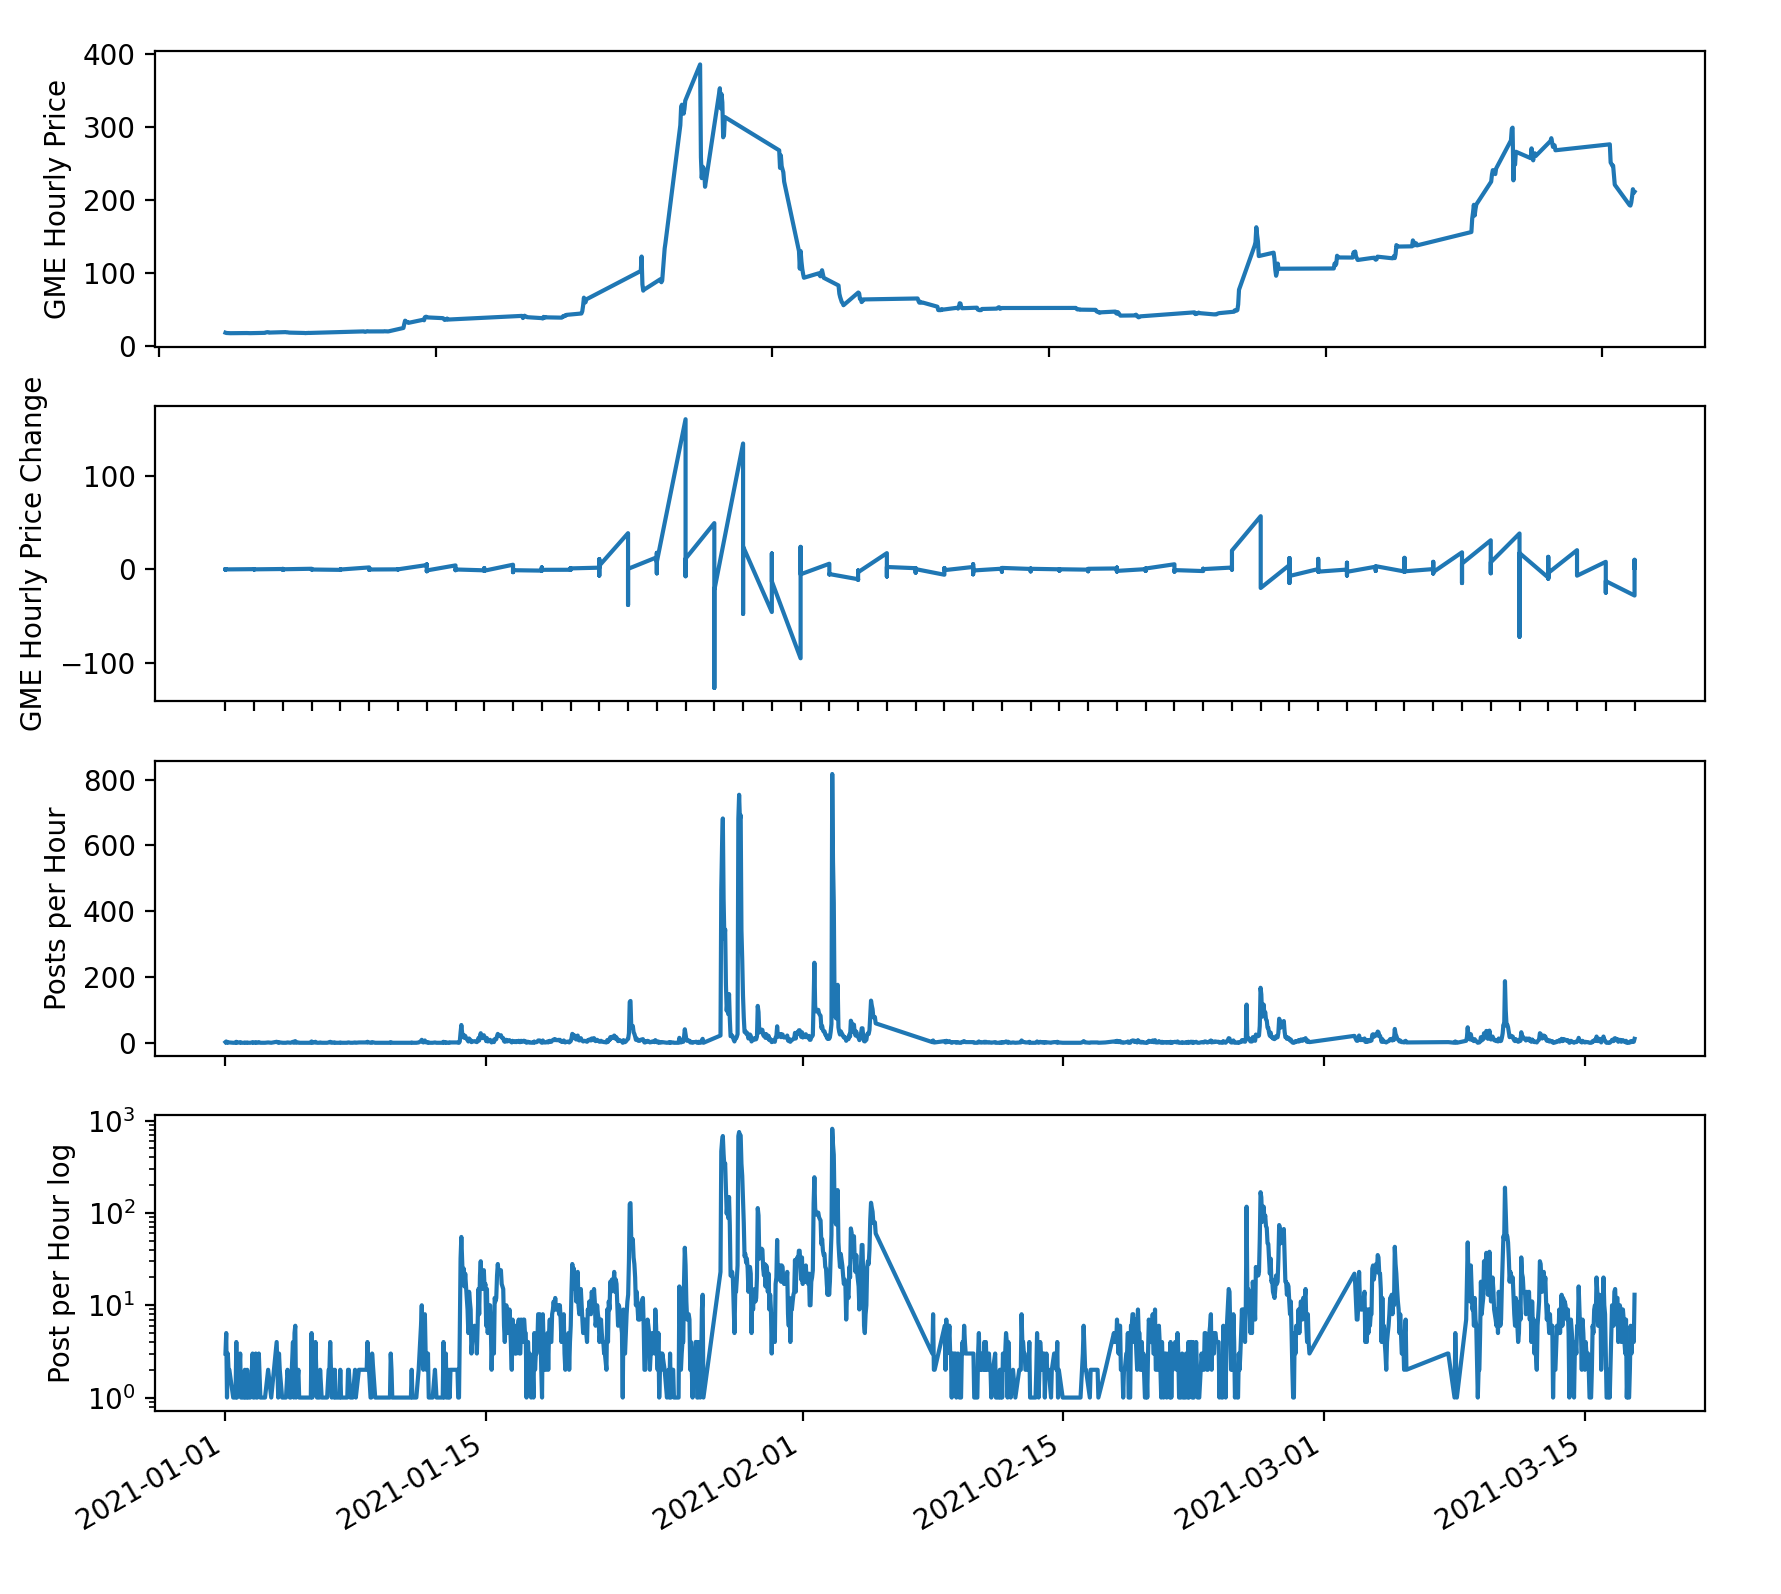
\includegraphics[width=0.9\linewidth]{figures/time_series.png}
    \caption{Time series of a) GME stock price hourly b) GME stock price hourly change c) number of post per time period d) log number of post per time period}
    \label{fig:posts_time}
\end{figure}


\end{document}
\endinput
%%
%% End of file `sample-authordraft.tex'.

